\section{Grundlagen des Testings}

Testing ist ein wichtiger Prozess bei der Entwicklung und Wartung von Software- und Hardwareprodukten. Das Hauptziel besteht darin, die Qualität, Sicherheit und 
Funktionalität des Produkts zu gewährleisten, indem Fehler und Probleme identifiziert werden, bevor das Produkt in Produktion geht oder an den Endbenutzer ausgeliefert wird. 
Zu den Hauptzielen des Testens gehören die Überprüfung der Einhaltung spezifizierter Anforderungen, die Validierung der Benutzererwartungen und die Identifizierung von 
Verbesserungsmöglichkeiten.

\paragraph{Testprozess}

Der Testprozess gliedert sich in mehrere Phasen, die eng miteinander verknüpft sind, um eine effiziente Überprüfung des Systems zu ermöglichen:

\begin{itemize}
    \item \textbf{Testplanung:} Diese Phase umfasst die Erstellung des Testkonzepts und des detaillierten Testplans. Hierbei werden das Testobjekt definiert, die erforderliche Testumgebung beschrieben, die Konfiguration des Testsystems festgelegt und die benötigten Testressourcen bestimmt. Die Testplanung legt den Grundstein für alle nachfolgenden Testaktivitäten und definiert den Umfang sowie die Werkzeuge, die für die Tests verwendet werden sollen.
    \item \textbf{Testdesign:} In dieser Phase werden die Testanforderungen verfeinert und spezifiziert. Es werden Testszenarien entwickelt und Kriterien für den Abschluss der Tests festgelegt. Je nach Umfang und Komplexität des Projekts kann diese Phase eng mit der Testplanung verbunden sein.
    \item \textbf{Testspezifikation:} Hier erfolgt die detaillierte Beschreibung der einzelnen Testfälle, einschließlich der Festlegung der Testvoraussetzungen, der Definition der Eingaben und der Spezifikation der erwarteten Ausgaben.
    \item \textbf{Testdurchführung:} Die Tests können manuell oder automatisiert durchgeführt werden, wobei häufig eine Kombination beider Methoden zum Einsatz kommt. Diese Phase ist typischerweise iterativ, um das System kontinuierlich zu testen und sicherzustellen, dass neue Funktionen und behobene Fehler keine unerwünschten Nebeneffekte verursachen (Regressionstests).
\end{itemize}

Der gesamte Testprozess ist dynamisch und passt sich den Gegebenheiten des jeweiligen Entwicklungsprojekts an. In agilen Umgebungen wird der Testprozess flexibel gestaltet, um schnell auf Änderungen reagieren zu können und eine gleichbleibend hohe Qualität zu gewährleisten. Das Testmanagement spielt dabei eine zentrale Rolle, indem es die verschiedenen Testaktivitäten koordiniert, Ressourcen verwaltet und die Kommunikation zwischen den Projektbeteiligten steuert. 

\paragraph{Grundsätze}
Im Rahmen von Tests sind einige Grundsätze zu berücksichtigen, die zu einem gemeinsamen Verständnis beitragen und eine korrekte Einordnung der Testaktivitäten ermöglichen. Im Folgenden erfolgt eine kurze Darstellung und Erläuterung ausgewählter Grundsätze:

Durch die Testaktivitäten werden Fehler erzeugt und somit erkannt. Je höher die Testabdeckung ist, desto geringer ist daher das Risiko, dass noch unentdeckte Fehler vorhanden sind. Testen kann jedoch nicht beweisen, dass ein System fehlerfrei ist. Ziel des Testens ist es daher, mit den gegebenen Ressourcen so viel Qualität wie möglich sicherzustellen.

Tests sind immer Stichproben. Es werden nicht alle möglichen Eingabemöglichkeiten mit allen möglichen Umgebungsbedingungen getestet, sondern häufig Grenzfälle oder Kombinationen, die am ehesten praxisrelevant sind. Der Aufwand hängt von der Priorität und dem Risiko ab und muss gegen den Nutzen des Tests abgewogen werden. Darüber hinaus dient ein Test dazu, festzustellen, ob ein System so funktioniert, wie es die Spezifikation vorsieht. Inwieweit diese Spezifikation sinnvoll ist, kann im Test hinterfragt werden, ist aber grundsätzlich nicht Aufgabe des Tests.

Es ist sinnvoll, frühzeitig mit dem Testen zu beginnen. Dadurch können Fehler bereits in der Entwicklungsphase erkannt werden, in der sie entstehen. Somit wird die Korrekturzeit verkürzt und der Integrationsaufwand verringert.

Häufig sind Fehler nicht gleichmäßig über das gesamte System verteilt, sondern treten gehäuft in bestimmten Komponenten auf. Daher sollte man beim Testen flexibel auf solche Häufungen eingehen und diese Bereiche genau überprüfen. Es ist also wichtig, neben einer genauen Testplanung auch kreativ auf solche Herausforderungen zu reagieren.

Neue Anforderungen, veränderte Umgebungsbedingungen und erweiterte Szenarien erfordern neue Testfälle. Die Testspezifikation muss ständig kritisch überprüft und gegebenenfalls ergänzt oder aktualisiert werden. Fehlende Tests führen zu einer unzureichenden Testabdeckung und damit zu einem erhöhten Fehlerrisiko.

Die Tests müssen an das Einsatzgebiet und die Umgebung des Systems angepasst werden. Die Testabdeckung und der Testumfang sind für jedes System individuell zu bewerten und festzulegen. Sicherheitskritische Systeme oder Anwendungen in der Medizin erfordern umfangreichere und detailliertere Tests als eine Spielsoftware oder eine grafische Benutzeroberfläche. Je nach Art der Anwendung unterscheiden sich auch die zu tolerierenden Fehler.

Grundsätzlich ist es sinnvoll, das Testen von der Entwicklung personell zu trennen, da eine andere Sichtweise auf das System erforderlich ist. Zudem bewertet ein Entwickler sein eigenes Produkt naturgemäß milder als ein neutraler Tester. So findet er tendenziell weniger Fehler und kann auch nicht korrigieren, wenn ein Fehler durch eine falsch verstandene Anforderung entstanden ist.

\paragraph{Testarten}

Die Überprüfung eines komplexen Systems gliedert sich in mehrere Testarten. Die Einordnung der Testarten orientiert sich an dem Entwicklungsstand des Systems. 
Dabei wird angestrebt, die Tests bestimmter Funktionalitäten möglichst frühzeitig durchzuführen. Abbildung \ref{fig:Testarten} zeigt eine Übersicht der verschiedenen 
Testarten sowie deren Eigenschaften in Bezug auf den Aufwand und die Anzahl der Testfälle:

\begin{figure}[htbp]
    \centering
      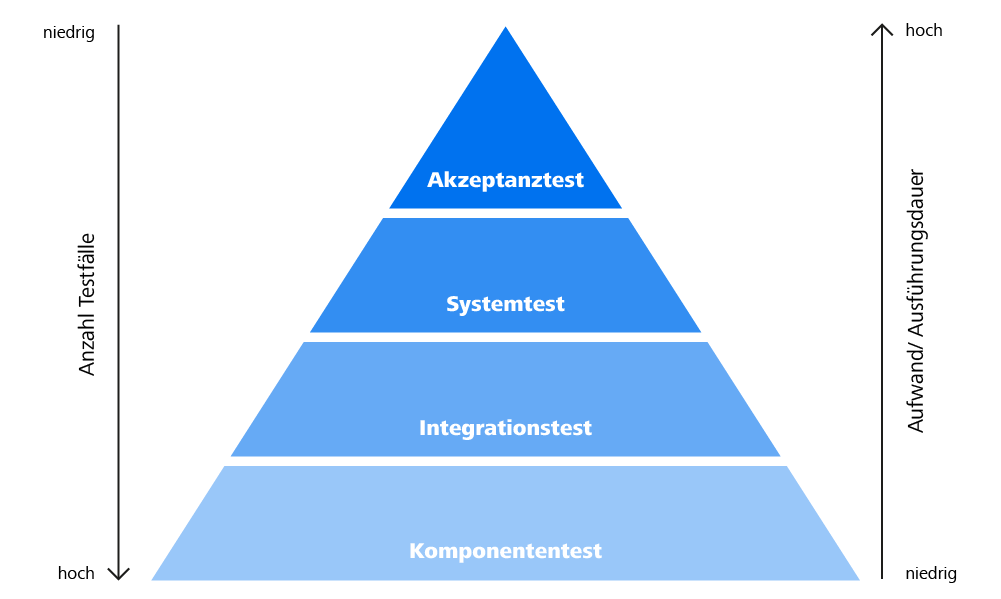
\includegraphics [width=0.75\textwidth]{Testarten.png}
    \caption[Testpyramide]{Testpyramide \citep{Zeiss2024}}
    \label{fig:Testarten}
\end{figure}

\begin{itemize}
    \item \textbf{Komponententests} (auch Modultests oder Unittests) werden durchgeführt, um die einzelnen Komponenten separat zu überprüfen.
    \item \textbf{Integrationstests} untersuchen, wie die verschiedenen Komponenten zusammenarbeiten und prüfen die Schnittstellen zwischen unterschiedlichen Systemen und Anwendungen.
    \item \textbf{Systemtests} erfolgen, wenn alle Komponenten zusammengeführt sind. Dabei wird die gesamte Anwendung auf die spezifizierten Anforderungen getestet.
    \item \textbf{Akzeptanztests} prüfen, ob die entwickelte Lösung die Anforderungen der Nutzer erfüllt. Sie werden in Zusammenarbeit mit dem Kunden durchgeführt und basieren auf zentralen Testfällen aus den Systemtests.
\end{itemize}

\citep{Witte2019} \citep{Witte2023}